\chapter{Introduction}
\head{In this chapter is the motivation for the project stated and the previous work within the subject will be summed up.}

\section{Motivation and the AAUSHIP Project}
The Port of Aalborg would like Aalborg University to help them to expand their options of improving the conditions of the Limfjord. One of their tasks is to map the seabed of the Limfjord to get bathymetry data. This will help them guide larger cargo ships to port while using the autonomous ships as guidance.

Another aspect from The Port of Aalborg is a task to escort larger ships with cargo into The Port of Aalborg. This is done by a pilot whom needs to sail out to incoming larger cargo ships and escort them safely into port. The pilot does this in a pilot boat which is controlled manually by the pilot. The Port of Aalborg would like this process to become autonomous such that an autonomous boat can sail to the cargo ship and to some extend take over the control and guide the cargo ship into port. The system to do this implies that The Port of Aalborg needs an autonomous ship which can perform this task.

The mapping itself can be done by one ship or by more. For the moment one of the ships from The Port of Aalborg, which is manned, and covers the mapping of the closer part of the Limfjord ($\approx$ 65 km). This is only done every third year, but mapping around Hals Barre (a sandbar and not a beach bar) at the end of the Limfjord is a more critical place and is mapped every third month.

If The Port of Aalborg had an autonomous ship fleet at their disposal, which could sail out and do the mapping autonomously, they would get updated bathymetry maps with a higher update frequency than they have currently \citep{portofaalborg}. This will result in a digitalizing of the seabed, a digital map, which has different implementation options by The Port of Aalborg.

This thesis will utilise formation control and extensions to manoeuvre agents through a specified area for surveying purposes. The aspect of formation control is chosen due to the rather large areas that The Port of Aalborg needs so cover. When applying formation control it is assumed to be faster to cover a larger area than if one single boat needed to scan the area. The formation that are to be chosen depends on the specific area of interest, which could e.g. be inside the harbour or around the pillars of the bridge. Chapter~\vref{ch:formcontrol} will introduce what kind and scopes of formation control that exists today. These theories makes the basis for the formation control within the scope of this project.

As a future scope this can be used when making a model of the seabed of how this will get sanded. This model can tell The Port of Aalborg when to go clean the seabed. The AAUSHIP project can be used to verify this model, such that The Port of Aalborg do not have to go out with equipment to solve the sanding without the need of it.

\section{The Mission}
\label{sc:mission}
Within the scope of this project the robots will be unmanned ships,
\ac{ASV}. The ship's main purpose will be to map the seabed by using
sonars to obtain bathymetry data. When one ship need to do this alone, and due to the range of
the sonar, the time spend could be improved by using multiple ships. The sonar scanning would
be done as seen on figure~\vref{fig:concept-art}.

\begin{figure}[htbp]
	\centering
	\subfloat[One ship\label{fig:concept-art1}]{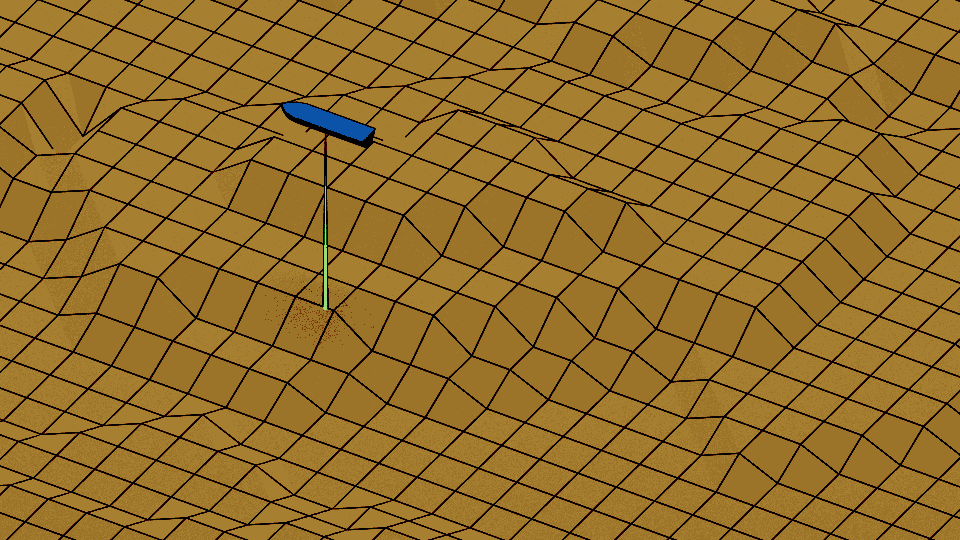
\includegraphics[width=0.48\textwidth]{fig/conseptart-single}}
	\ % One forced space to seperate figures
	\subfloat[Thee ships\label{fig:concept-art3}]{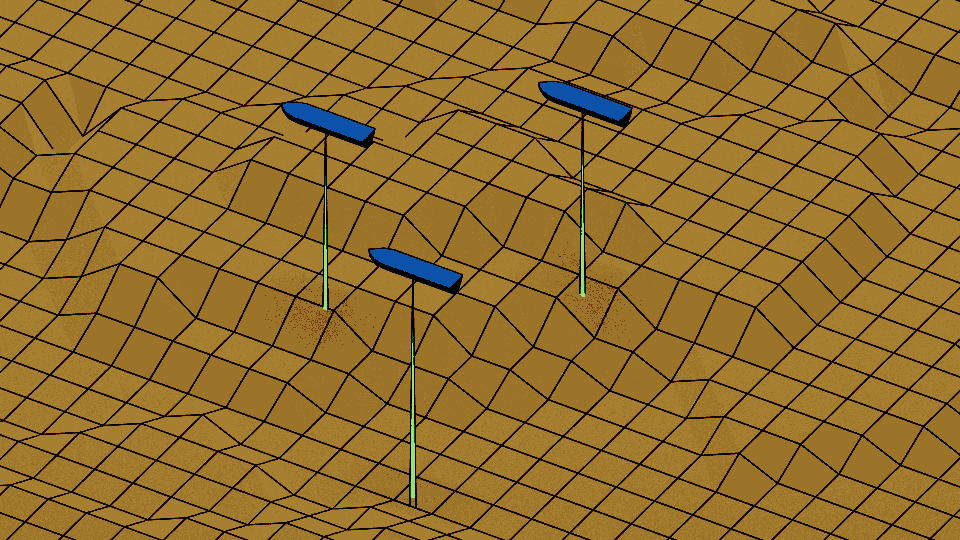
\includegraphics[width=0.48\textwidth]{fig/conseptart-formation}}
	\caption{Comparison of two ways to cover an area with a lawn mower
	pattern.}
	\label{fig:concept-art}
\end{figure}


When only one ship (figure~\vref{fig:concept-art1}) need to map a complete seabed this process could
take up much time dependent on the area that need to be covered. The
time spend could be improved to make this mapping more efficient. One
way of optimizing the time used is to add more ships (figure~\vref{fig:concept-art3}) to help map the
seabed. To make the process of this as optimal as possible it could be
of benefit to implement formation control in the specific assignment.

I cooperation with the port of Aalborg, a use case is presented, where we can perform tests of the platform, and use those to compare the performance of our system to their system.
\begin{figure}[htbp]
	\centering
	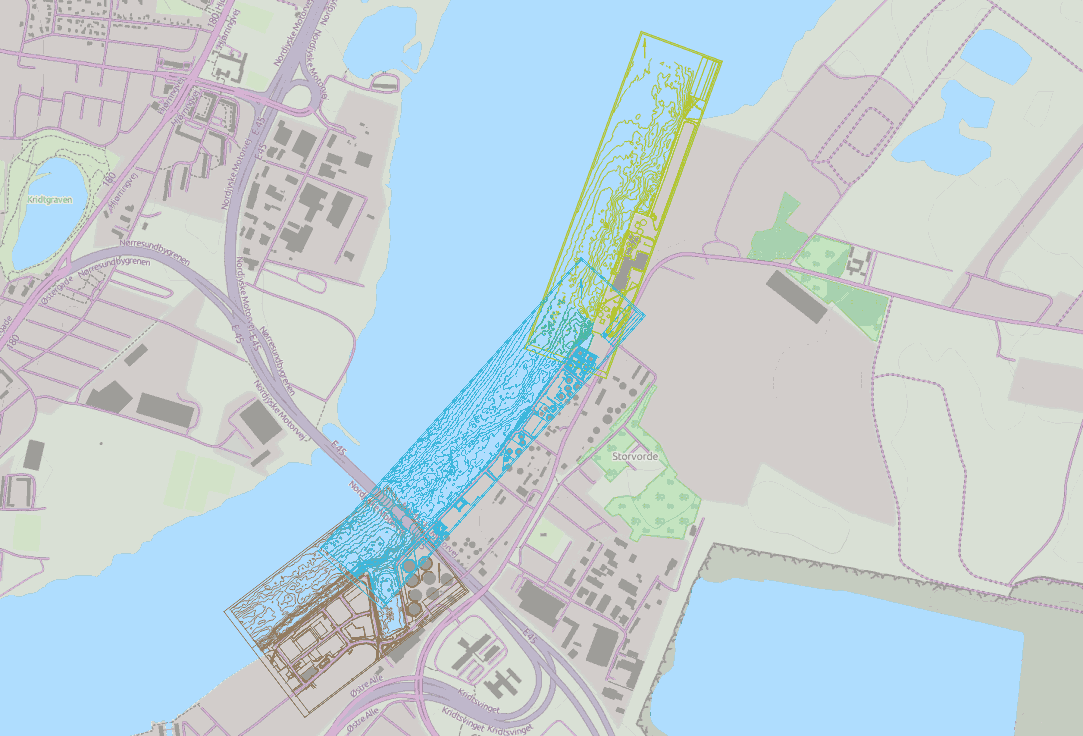
\includegraphics[width=\textwidth]{fig/use-case-data}
	\caption{Area of the harbour at Aalborg Portland provided as sample
	data from Aalborg Havn. Background map data CC BY-SA OpenStreetMap.}
	\label{fig:diffforms}
\end{figure}

When performing this kind of surveying with multiple ships, it is important to take note of the kind of sensor it uses and the coverage that it provides. Initially the port of Aalborg used single beam echo sounders, but have in recent years turned over to multibeam sonars for their survey boat, which has improved their resolution and time for a survey. But they still wishes to improve the survey update rate, by e.g. using fairly low cost autonomous ships to get better indication of the seabed to identify if an expensive thorough survey is needed. An image of the survey vessel they use now used can be seen on figure \ref{fig:alba}. As it can be seen, this survey vessel is relatively large, being over 20 metres long. To comparison is the AAUSHIP only 1.1 metres long. For surveying in smaller areas, like inside the harbour area, Aalborg Havn uses a smaller scale vessel which is 12 metres long. This vessel is only used at the smaller areas thus not the one being used out in the Limfjord close to Aalborg.
\begin{figure}
	\centering
	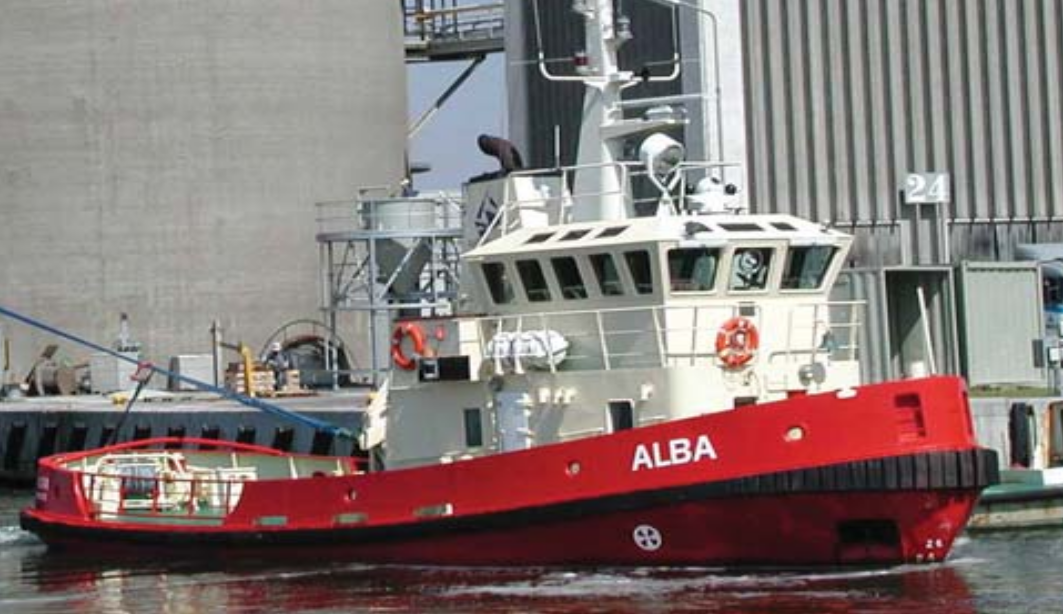
\includegraphics[width=0.6\textwidth]{fig/alba}
	\caption{The survey vessel used by Aalborg Havn named Alba.}
	\label{fig:alba}
\end{figure}



%This could be done in several ways, but is mostly thought of in a
%rigid formation, such that the formation maps the same area of the
%seabed the whole time. The idea can be seen on
%figure~\vref{fig:concept-art}.
